% !TeX root = ../../../main.tex

The main input to our determination of intrinsic charm is the 4\fns
charm \pdf extracted from high-energy data. While this
determination comes with an uncertainty estimate, it is important to
verify that this adequately reflects the various sources
of uncertainty, and that there are no further sources of uncertainty
that may be unaccounted for.
%
To this purpose, here we assess the
stability of our results first, upon the choice of underlying dataset,
next upon changes in methodology, and finally, upon variation of
standard model parameters.
%
In each case we verify stability upon the
most important possible source of instability: respectively, the use
of collider vs.\ fixed target and deep-inelastic vs.\ hadronic data
(dataset); the choice of parametrization basis (methodology); and the
value of the charm quark mass (standard model parameters).
%
As a final consistency check, we compare our result with that which we
would have obtained by using the same input dataset, but the previous
NNPDF3.1 fitting methodology.
%
Because we
are interested in intrinsic charm, in all comparisons we focus on
the large-$x$ region in which the intrinsic valence-like peak is found.
%
In this section, the 4\fns
charm \pdf is displayed at the scale $Q = 1.65$ GeV so that
results for all fit variants, including
those with with different $m_c$ values, can be shown at a common scale.

\paragraph{Dependence on the choice of dataset.}
%
We now study the stability of the  4\fns charm determination upon
variation of the
underlying data, which also allows us to
identify the datasets or groups of processes that provide
the leading constraints on intrinsic charm.
%
To this purpose, we have repeated our \pdf
determination using a  variety of subsets of the global dataset used for
our default determination. Results are shown in
Fig.~\ref{fig:ic/charm_dataset_dep}, where we compare the result using
the 
baseline dataset to determinations performed by adding to the baseline
the  \emc charm
structure function data (already discussed in the main text); by only
including  DIS data; by only including collider data (HERA,
Tevatron and \lhc); and by removing the \lhcb  $W$ and $Z$ production data.

%%%%%%%%%%%%%%%%%%%%%%%%%%%%%%%%%%%%%%%%%%%%%%%%%%%%%%%%%%%%%%%%%%%
\begin{figure}[t!]
  \begin{center}
    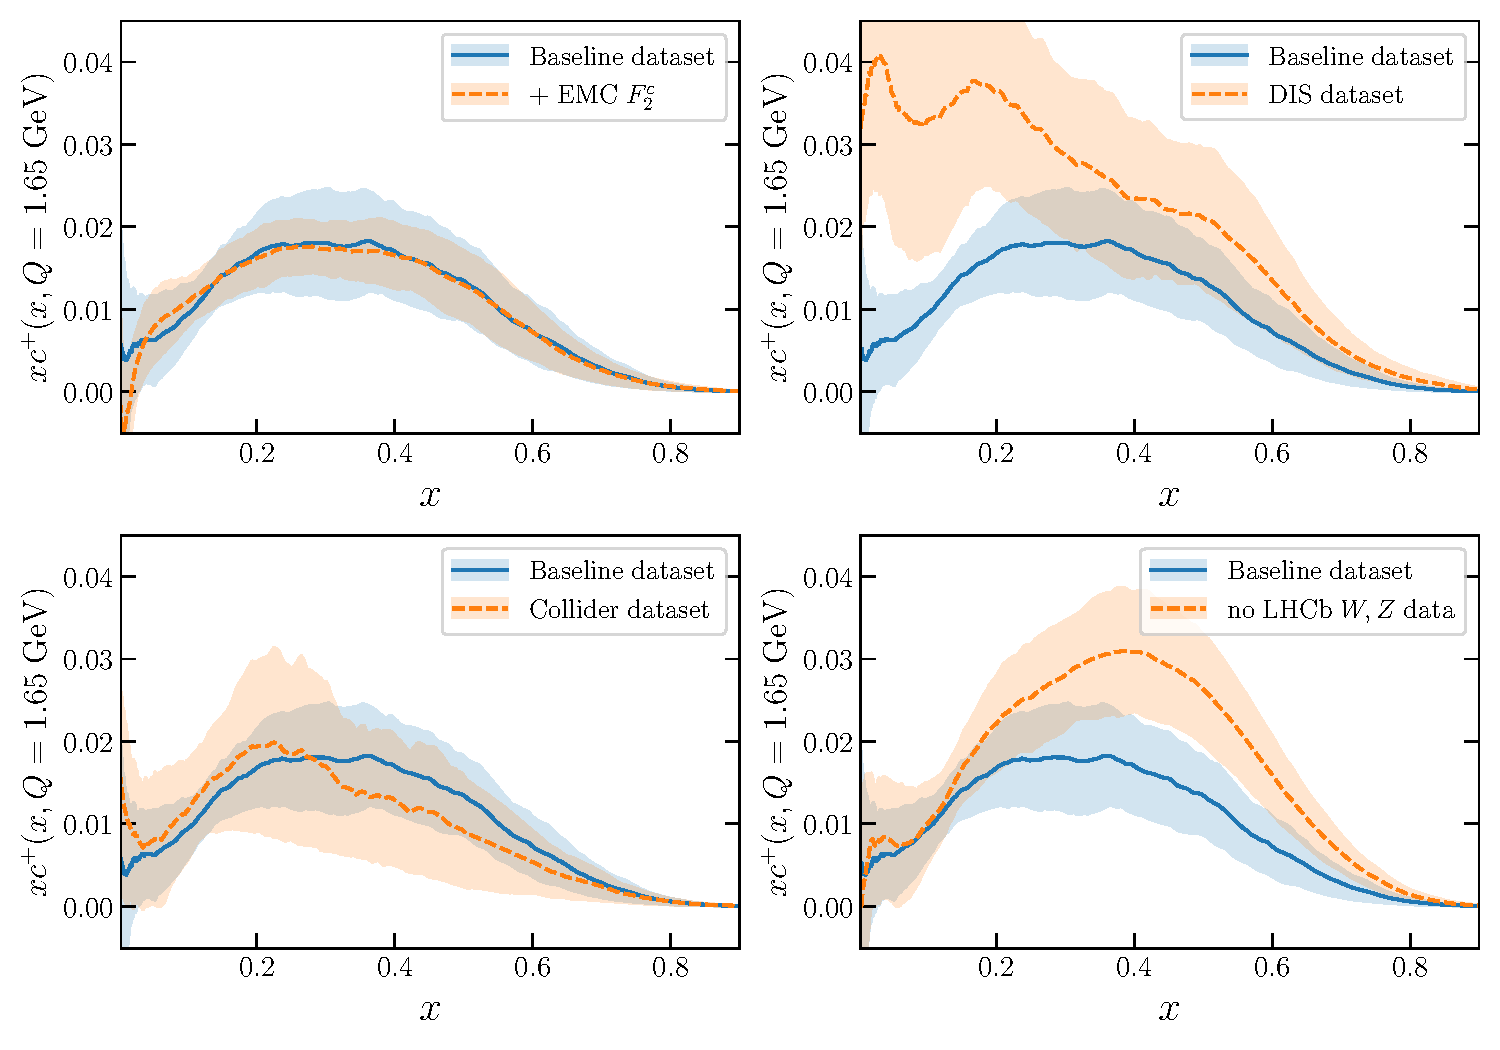
\includegraphics[width=0.99\linewidth]{ch-ic/pdfplot-abscharm-dataset_dep.pdf}
    \caption{\small The dependence of the 4\fns charm \pdf at $Q=1.65$ GeV on
      the input dataset.
      %
      We compare the
    baseline result with that obtained by also including 
      \emc $F_2^c$ data (top left), only including DIS data (top
    right), only including collider data (bottom left) and removing
    \lhcb gauge boson production data (bottom right). 
  \label{fig:ic/charm_dataset_dep} }
\end{center}
\end{figure}
%%%%%%%%%%%%%%%%%%%%%%%%%%%%%%%%%%%%%%%%%%%%%%%%%%%%%%%%%%%%%%%%%%%%%%

As already noted in the main  text in the case of the 3\fns
result, we find that the extra information provided by the  \emc
$F_2^c$ data is subdominant in comparison to that from the global
dataset. The result is stable and only a moderate
uncertainty reduction at the peak is observed. It is interesting to
contrast this with the previous NNPDF study~\cite{Ball:2016neh}, in
which the global fit provided only very loose constraints on the charm
\pdf, which was then determined mostly by the \emc data.
%
Indeed, a DIS-only fit (for which most data were already available at the time
of the previous determination) determines charm with very large
uncertainties. On the other hand, both the central value and
uncertainty found in the collider-only fit are quite similar to the
baseline result.
%
This shows that the dominant constraint is now coming from
collider, and specifically hadron collider data (indeed, as we have
seen constraints from DIS data are quite loose). Among these, \lhcb
data (which are taken at large rapidity and thus impact \pdfs at large
and small $x$) are especially important, as demonstrated by the
increase in uncertainty when they are removed.

In all these determinations, the charm
\pdf at $x\simeq 0.4$ remains consistently nonzero and positive, thus
emphasizing the stability of our results.

\paragraph{Dependence on the parametrization basis.}
%
Among the various methodological choices, a possibly critical one is
the choice of basis functions. Specifically, in our default analysis,
the output of the neural network does not provide the individual
quark flavor and antiflavor \pdfs, but rather linear combinations
corresponding to the so-called evolution
basis~\cite{Ball:2021leu}. Indeed, our charm \pdf is given in
Eq.~(\ref{eq:ic/fitted_charm_param})  as the linear combination of the
two basis \pdfs $\Sigma$ and $T_{15}$.
One may thus ask whether this choice may influence the final results
for individual quark flavors, specifically charm.
Given that physical results are basis
independent, the outcome of a \pdf determination should not depend
on the basis choice.

In order to check this, we have repeated the \pdf determination, but
now using the flavor basis, see Sect.~3.1 of~\cite{Ball:2021leu}, in which
each of the  neural network output neurons now correspond to individual quark
flavors, so in particular,
instead of Eq.~(\ref{eq:ic/fitted_charm_param}),  one has
\begin{equation}
\label{eq:ic/fitted_charm_param_flavour}
xc^+(x,Q_0;{\boldsymbol \theta}) =
 (1-x)^{\beta_{c^+}} \textrm{ NN}_{c^+}(x,{\boldsymbol \theta}) \, ,
\end{equation}
where $\textrm{ NN}_{c^+}(x,{\boldsymbol \theta})$
indicates the value of the output neuron associated to the charm \pdf $c^+$.
%
The 4\fns charm \pdfs determined using either basis are compared 
in Fig.~\ref{fig:ic/charm_basisdep}  at $Q=1.65$ GeV.
%
We find excellent consistency, and in particular 
the valence-like structure at high-$x$ is independent of the choice
of parametrization basis.

%%%%%%%%%%%%%%%%%%%%%%%%%%%%%%%%%%%%%%%%%%%%%%%%%%%%%%%%%%%%%%%%%%%
\begin{figure}[t!]
  \begin{center}
    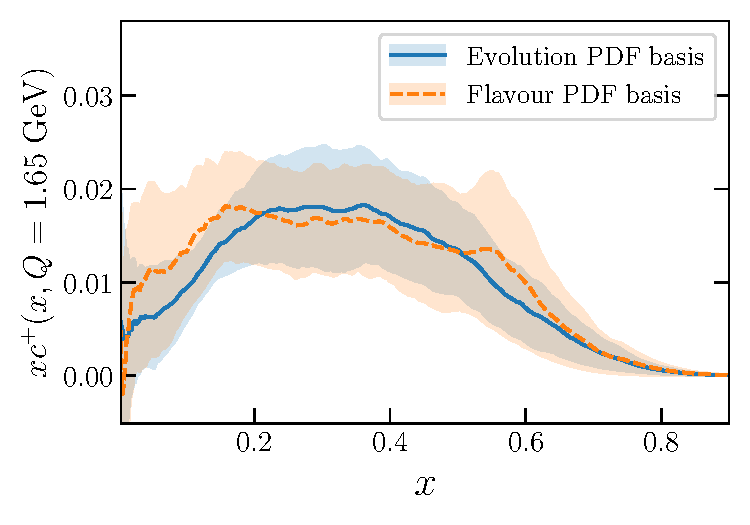
\includegraphics[width=0.60\linewidth]{ch-ic/pdfplot-abscharm-basisdep.pdf}
    \caption{\small The default 4\fns charm \pdf at $Q=1.65$ GeV
    compared to a result obtained by parametrizing \pdfs in the flavor
    basis instead of the evolution basis. 
  \label{fig:ic/charm_basisdep} }
\end{center}
\end{figure}
%%%%%%%%%%%%%%%%%%%%%%%%%%%%%%%%%%%%%%%%%%%%%%%%%%%%%%%%%%%%%%%%%%%%%%

\paragraph{Dependence on the charm mass.}
%
The kinematic threshold for producing charm perturbatively depends on
the value of the charm mass. Therefore the perturbative contribution
to the 4\fns charm \pdf, and thus the whole charm \pdf if one assumes
perturbative charm, depends strongly on the value of the charm
mass.
On the other hand, the intrinsic charm \pdf is of nonperturbative
origin, so it should be essentially independent of the numerical value of the
charm mass that is used in  perturbative computations employed in  its 
determination (though it will of course depend on the true underlying 
physical value of the charm mass).

In order to study this mass dependence, we have repeated our determination using different values for the charm mass.
The definition of the charm mass which is relevant for kinematic
thresholds is the pole mass, for which we adopt the value recommended
by the Higgs cross-section working group~\cite{deFlorian:2016spz}
based on the study of~\cite{Bauer:2004ve}, namely
 $m_c = 1.51 \pm 0.13$~GeV. 
%
Results are shown in Fig.~\ref{fig:ic/charm_fitted_mcdep}, where
our default charm \pdf determination with  $m_c = 1.51$~GeV is
repeated with $m_c=1.38$~GeV and
$m_c=1.64$~GeV.
%
In order to understand these results note that this is
the 4\fns \pdf, so it includes 
both a nonperturbative and a perturbative component. The latter is
strongly dependent on the charm mass, but of course the data
correspond to the unique true value of the mass and the mass
dependence of the perturbative component is present only due to our
ignorance of the actual true value. When determining the \pdf from the
data, as we do, we expect this spurious dependence to be to some extent
reabsorbed into the fitted \pdf. So we expect results to display a
moderate dependence on the charm mass --- full independence should
hold for the intrinsic (3\fns) \pdf and will be investigated in
SI Sect.~\ref{sec:ic/charm_stability_3fns}. 

In Fig.~\ref{fig:ic/charm_pert_mcdep} the same result is shown, but now
for the perturbative charm \pdf discussed in
SI Sect.~\ref{sec:ic/consistency},  so the charm \pdf is of
purely perturbative origin and fully determined by the strongly
mass-dependent matching condition. This dependence is clearly seen in
the plots. Furthermore, comparison with
Fig.~\ref{fig:ic/charm_fitted_mcdep} shows that indeed this spurious
dependence is partly reabsorbed in the fit when the charm \pdf is
determined from the data, so that  the residual mass dependence is moderate.
In particular, the large-$x$ valence peak, which is dominated by the
intrinsic component, is very stable.

%%%%%%%%%%%%%%%%%%%%%%%%%%%%%%%%%%%%%%%%%%%%%%%%%%%%%%%%%%%%%%%%%%%
\begin{figure}[t]
  \begin{center}
    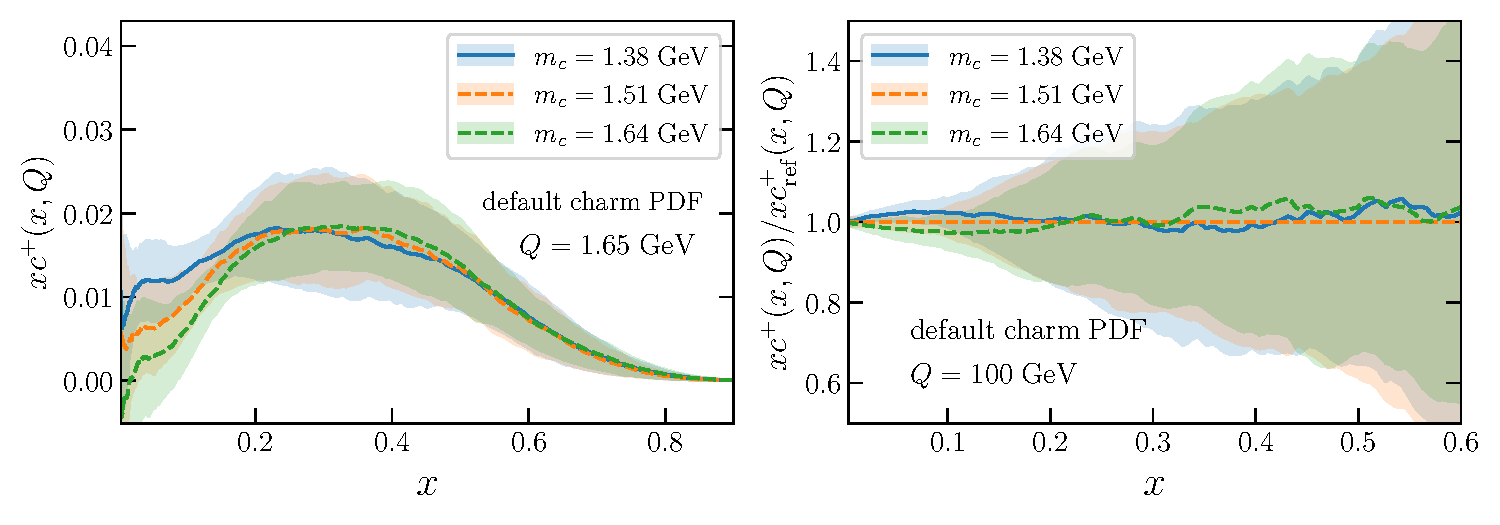
\includegraphics[width=0.99\linewidth]{ch-ic/pdfplot-abscharm-mcdep.pdf}
    \caption{\small The 4\fns charm \pdf determined
    using three different values of the charm mass. The absolute
    result (left) is shown at $Q=1.65$ GeV, while the ratio to the 
       default value
       $m_c=1.51$~GeV (right) used elsewhere in this paper is shown at $Q=100$ GeV.
   \label{fig:ic/charm_fitted_mcdep} }
\end{center}
\end{figure}
%%%%%%%%%%%%%%%%%%%%%%%%%%%%%%%%%%%%%%%%%%%%%%%%%%%%%%%%%%%%%%%%%

%%%%%%%%%%%%%%%%%%%%%%%%%%%%%%%%%%%%%%%%%%%%%%%%%%%%%%%%%%%%%%%%%%%
\begin{figure}[t]
  \begin{center}
    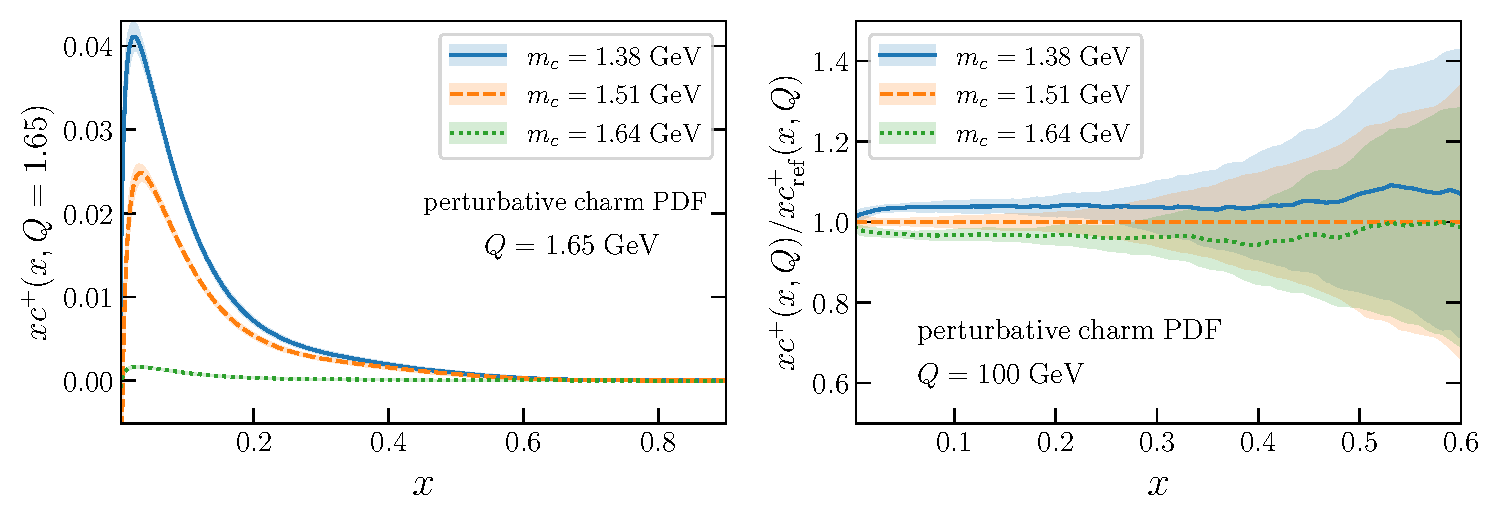
\includegraphics[width=0.99\linewidth]{ch-ic/pdfplot-abscharm-mcdep-highQ.pdf}
    \caption{\small The same as Fig.~\ref{fig:ic/charm_fitted_mcdep} but now
    for the perturbative charm \pdf.
  \label{fig:ic/charm_pert_mcdep} }
\end{center}
\end{figure}
%%%%%%%%%%%%%%%%%%%%%%%%%%%%%%%%%%%%%%%%%%%%%%%%%%%%%%%%%%%%%%%%%



  \paragraph{Comparison with NNPDF3.1.}
  %
  Fig.~\ref{fig:ic/pdfplot-abscharm-40-vs-31meth} compares
  the baseline determination of the 4\fns charm \pdf based
  on NNPDF4.0 with that obtained
  from the same input dataset but using instead
  the NNPDF3.1 fitting methodology and related settings such those related to positivity
  and integrability.
  %
  Results are fully consistent between the two methodologies, with our default
  determination exhibiting reduced uncertainties due to
  the various improvements implemented
  in the NNPDF4.0 analysis framework.
  
%%%%%%%%%%%%%%%%%%%%%%%%%%%%%%%%%%%%%%%%%%%%%%%%%%%%%%%%%%%%%%%%%%%
\begin{figure}[t]
  \begin{center}
    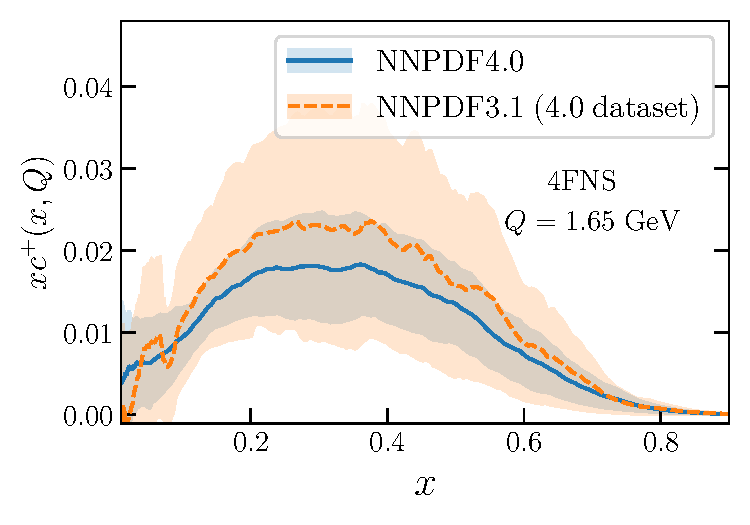
\includegraphics[width=0.65\linewidth]{ch-ic/pdfplot-abscharm-40-vs-31meth.pdf}
    \caption{\small Same as Fig.~\ref{fig:ic/charm_basisdep}, comparing
      the baseline determination of the 4\fns charm \pdf, based
      on NNPDF4.0, with that obtained
      from the same dataset using the NNPDF3.1 fitting methodology.
  \label{fig:ic/pdfplot-abscharm-40-vs-31meth} }
\end{center}
\end{figure}
%%%%%%%%%%%%%%%%%%%%%%%%%%%%%%%%%%%%%%%%%%%%%%%%%%%%%%%%%%%%%%%%%

